\documentclass{CSICC}

% تقریبا تمامی بسته‌های مورد نیاز برای یک مقاله در استایل فراخوانی شده است. اما در هر صورت در صورتی‌که می‌خواهید بسته‌ای را فراخوانی کنید به صورت زیر عمل کنید. مثلا ما در کد زیر دوبسته glossaries و tikz را فراخوانی کرده‌ایم.
%\makeatletter
%\bidi@BeforePackage{xepersian}{
%\RequirePackage{tikz}
%\RequirePackage{glossaries}
%}
%\makeatother


% عنوان مقاله را در این قسمت وارد کنید. 
\title{
راهنمای نوشتن مقاله در کنفرانس انجمن کامپیوتر ایران
}
\date{}
% اسامی نویسندگان و همچنین اطلاعات مربوط به آن‌ها را در این قسمت وارد کنید. 
\author[1]{نام و نام خانوادگی نویسنده اول}
\author[1]{نام و نام خانوادگی نویسنده دوم}
\author[1,2]{نام و نام خانوادگی نویسنده سوم}
\affil[1]{
 رتبه علمی نویسنده در صورت تمایل، گروه آموزشی یا واحد سازمانی مربوطه، نام سازمان ، شهر،
آدرس پست الکترونیکی
}
\affil[2]{
 رتبه علمی نویسنده در صورت تمایل، گروه آموزشی یا واحد سازمانی مربوطه، نام سازمان ، شهر،
آدرس پست الکترونیکی
}


\begin{document}
\maketitle
\begin{abstract}
در این مقاله، شیوه نگارش یك مقاله برای بیست و یکمین كنفرانس ملی سالانه انجمن کامپیوتر ایران تشریح می‌شود. روش قالب‌بندی مقاله، بخش‌های مختلف آن، انواع قلم‌ها و اندازه آن‌ها، به طور كامل مشخص شده است. كلیه سبك (\lr{Style}) های مورد نیاز برای بخش‌های مختلف مقاله، از جمله عنوان‌ها، نویسندگان، چكیده، متن، و ... از پیش تعریف شده‌اند. نویسندگان محترم مقاله‌ها باید توجه داشته باشند، كنفرانس از پذیرش مقاله‌هایی كه خارج از این چارچوب تهیه شده باشند، معذور است. چكیده مقاله باید در یك یا دو بند (پاراگراف) تهیه شود و حداكثر شامل 200 كلمه باشد. چكیده باید بطور صریح و شفاف موضوع پژوهش و نتایج آن را مطرح كند؛ یعنی بیان كند چه كاری، چگونه، و برای چه هدفی انجام و چه نتایجی حاصل شده است. در چكیده از ذكر جزییات كار، شكل‌ها، جدول­ها، فرمول‌ها، و مراجع‌ پرهیز كنید.
 \end{abstract}
\begin{keywords}
حداكثر 10 كلمه بعنوان كلمات كلیدی انتخاب شود. این كلمات باید موضوعات اصلی و فرعی مقاله را نشان دهند. بین هر کلمه کلیدی با علامت ویرگول (،) جدا گردد. در پایان آخرین کلمه کلیدی، نیز نقطه گذاشته‌شود. 
\end{keywords}

\section{مقدمه}
نویسندگان مقالات می‌توانند از استایل \lr{\LaTeX} تهیه شده برای نوشتن مقالات خود استفاده کنند. نویسندگان نباید به هیچ‌وجه اندازه فونت، حاشیه، ستون‌ها، فاصله بین ستون‌ها و ... تنظیم شده در استایل را تغییر دهند. حداکثر تعداد صفحات مقاله  شما با استفاده از این استایل نباید از شش صفحه تجاوز کند. این شش صفحه شامل متن اصلی، تصاویر، جداول، مراجع، پیوست‌ها و هرچیز دیگری است. نکاتی که در ادامه خواهد دید، در حقیقت تعیین کننده سبک کلی مقاله است. شما نیازی نیست نگران اعمال بسیاری از این نکات باشید، چراکه تمامی آن‌ها در استایل \lr{\LaTeX} قرار داده شده وجود دارد و از قبل تعیین شده است.
\begin{itemize}
\item 
اندازه صفحات \lr{A4} و حاشیه‌های بالا، پایین، چپ، و راست هر صفحه به ترتیب برابر با 
$25mm$، $25mm$، $20mm$، و $20mm$
انتخاب شود. (فقط حاشیه بالای اولین صفحه، 5 سانتی‌متر انتخاب شود).
\item
فاصله بین خطوط نیز در این راهنما و سبک‌های آن تعریف شده است که حالت Single با Before و After صفر (0) است.
\item
مقالات باید به صورت دو ستونی تهیه شود. عرض هر ستون برابر $8.2$ سانتی‌متر و فاصله بین دو ستون $0.6$ سانتی‌متر است.
\item
 برای قلم لاتین همواره از \lr{Times New Roman} استفاده كنید. اندازه قلم لاتین یك واحد كمتر از اندازه قلم پارسی در هر موقعیت است. برای قلم پارسی هم از قلم میترا  که نام فایل آن \lr{IRMitra} است، استفاده نمایید. این فونت استاندارد را می‌توانید از سایت زیر بارگیری کنید:

\href{http://www.scict.ir/portal/File/ShowFile.aspx?ID=8964a122-b392-4261-9dd5-10c1938f0c8a}{
سایت دبیرخانه شورای عالی اطلاع‌رسانی- ۳۹ فونت استاندارد
}

در ضمن این فونت در پوشه‌ای به نام \lr{Font} به همراه استایل قرار داده شده است. دقت کنید که کاربران \lr{\LaTeX} می‌بایست این قلم را ابتدا بر روی رایانه خود نصب کنند تا بتوانند کامپایل موفقی از استایل تهیه شده بگیرند. 
\item
صفحه اول مقاله باید كاملاً مشابه صفحه اول این مقاله باشد. در صفحه اول از نوشتن سایر موارد خودداری كنید. همچنین تمام موارد صفحه اول باید در همان صفحه آماده و نوشته شوند.
\item
از شماره‌گذاری صفحات و بكاربردن سرصفحه و پاصفحه خودداری كنید.
\end{itemize}


\section{بخش‌بندی مقاله}
هر مقاله باید شامل این بخش‌های اصلی باشد: چكیده، كلمات كلیدی، مقدمه، مطالب اصلی، نتیجه‌گیری، و مراجع. سایر بخش‌ها مثل سپاسگزاری، پیوست‌ها و زیرنویس‌ها اختیاری است. این بخش‌ها باید در آخر مقاله و قبل از مراجع قرار گیرند، بجز بخش زیر‌نویس‌ها كه پس از مراجع آورده می‌شود.


شماره‌گذاری بخش‌ها از مقدمه شروع می‌شود. مقدمه دارای شماره 1 است. آخرین شماره نیز مربوط به بخش نتیجه است. سایر بخش‌های قبل از مقدمه و پس از نتیجه گیری (به جز بخش پیوست)، دارای شماره نیستند. هر بخش می‌تواند شامل چند زیربخش باشد. زیربخش‌ها نیز دارای شماره هستند كه از 1 شروع می‌شود. هنگام شماره‌گذاری زیربخش‌ها دقت كنید كه شماره بخش در سمت راست قرار گیرد. البته توصیه می‌شود کاربرانی که از \lr{\LaTeX} استفاده می‌کنند ترجیحا برای ارجاع به شماره بخش‌ها از تعریف برچسب و دستور \lr{ref} استفاده کنند. به عنوان مثال برای شماره‌گذاری زیربخش 3 از بخش 2 بنوسید
\ref{IntroMainFeat}.

در هر بخش یا زیربخش یك یا چند بند (پاراگراف) وجود دارد. دقت شود كه جملات هر بند زنجیروار به هم مربوط باشند و یك موضوع را دنبال كنند. اولین بند هر بخش یا زیربخش بدون تورفتگی (\lr{Intend}) است. این کار در \lr{\LaTeX} به صورت خودکار انجام می‌شود و لازم نیست نویسندگان درگیر جزئیات آن شوند. 

\subsection{ویژگی­های عنوان و نویسندگان مقاله}
عنوان مقاله در عین كوتاهی باید تمام ویژگی‌های كار پژوهشی را نشان دهد. عنوان مقاله را در یك یا دو سطر  بنویسید. 
پس از عنوان مقاله باید نام نویسندگان مقاله نوشته شوند. در هنگام نوشتن نام نویسندگان از ذكر عناوینی مثل استاد، دكتر، مهندس، و ... خودداری كنید. در صورت تمایل می‌توانید سِمت یا مرتبه علمی هر نویسنده را به شكل زیرنویس تهیه كنید. همچنین نام دانشگاه یا محل اشتغال نویسنده به همراه نشانی، تلفن تماس، و نشانی رایانامه می‌تواند ذكر شوند. 

\subsection{ویژگی­های چكیده و كلمات كلیدی}
چكیده مقاله باید بطور صریح موضوع و نتایج كار پژوهشی انجام شده را بیان كند. در چكیده تنها باید به اصل موضوع مقاله توجه شود و در آن از ذكرجزییات كار، شكل‌ها، جدول‌ها، فرمول‌ها، و مراجع خودداری شود. چكیده را حداكثر در 200 كلمه و در یك یا دو بند (پاراگراف) تهیه كنید. 

برای هر مقاله حداكثر 10 كلمه كلیدی انتخاب كنید، و آنها را با ویرگول از هم جدا كنید. این كلمات باید موضوعات اصلی و فرعی مقاله را دسته‌بندی كنند. كلمات كلیدی را به ترتیب وابستگی مقاله به آنها بنویسید؛ یعنی كلماتی كه مرتبط‌تر هستند، اول نوشته شوند. اگر از مختصر‌نویسی در چكیده یا كلمات كلیدی استفاده شده است، باید شكل كامل آن در داخل یك جفت هلالین (پرانتز) آورده شود.

\subsection{ویژگی­های مقدمه}
\label{IntroMainFeat}
در بخش مقدمه مقاله، باید چهار قسمت اصلی حتما وجود داشته‌باشد. در قسمت اول به صورت مقدمه‌وار، نویسنده مقاله باید در مورد حوزه‌ای که می‌خواهد بر روی آن کار کند، توضیحات مقدماتی را ارایه کند. در این قسمت تلاش می‌شود خواننده با کلیت موضوع آشنا شود. در قسمت دوم که انگیزش نام دارد، نویسنده باید به صورت صریح بیان کند که چه عاملی موجب انگیزش او برای کار کردن بر روی این موضوع بوده است. در این قسمت هدف از کار انجام شده تبیین می‌شود و به طور مشخص کاربردهایی که می‌توانند محملی عملی برای استفاده از کار انجام شده  توسط محقق باشند، ذکر می‌شود. به طور مشخص می‌توان یک مثال انگیزاننده  را مطرح کرد  و بدین سان به خواننده طرحی کلی از هدف نهایی کار و کاربرد آن ارائه داد. در مثال انگیزاننده  می‌توان به مقدار بسیار جزیی وارد نتایج دست‌یافته پیشین در مورد آن مثال خاص و تاریخچه آن اشاره داشت. در قسمت سوم نویسندگان باید نوآوری‌های مقاله را به صورت صریح و دقیق بیان کنند. بهتر است که به منظور تصریح بیشتر، نوآوری‌های مقاله به صورت شماره‌گذاری شده و یا آیتم‌بندی شده ذکر شود. به عنوان مثال نمونه زیر را در نظر بگیرید. 
\begin{itemize}
\item
در این مقاله ما یک مدل ریاضی برای مدل‌سازی رفتار کاربر ... .
\item
ارایه یک روش نوین به منظور بهبود کارایی شبکه در حضور ... .
\item
تحلیل و ارزیابی روش پیشنهادی با ارایه یک ....
\end{itemize}
در قسمت آخر نیز باید ساختار مقاله و فهرستی از مطالبی که در بخش‌های آینده وجود دارد، ارایه شود. دقت کنید که در این قسمت باید به بخش‌های بعدی مقاله در حد یک جمله اشاره‌ای کوتاه شود.

\subsection{ویژگی‌های بخش مروری بر کارهای پیشین}
در این بخش نویسندگان می‌بایست مروری بر کارهای صورت پذیرفته در موضوع مقاله داشته‌باشند. در این بخش مقالاتی باید مورد بررسی قرار گیرد که از یک اعتبار به نسبت بالا برخوردار باشد.  ملاک معتبر بودن مقاله ارجاع‌های آن بالا باشد و یا در مجله و کنفرانس‌های معتبر چاپ شده باشند.  در ضمن نویسندگان حتما باید مقالات مربوط به سال‌های اخیر را نیز مورد بررسی قرار دهند. 

معمولا در حوزه مقاله کار‌های فراوانی انجام شده که نویسنده موظف است به آنها اشاره داشته باشد. این مهم ممکن است در این بخش قابل بیان نباشد و نیاز به شاخه بندی کارها تحت عنوان زیربخش‌هایی باشد. مثلا فرض کنید در یک مقاله می‌خواهیم یک الگوریتم پیش‌گیری از ازدحام ارائه کنیم. در قسمت کارهای مرتبط می‌توان به زیر بخش‌هایی تقسیم کرد و در هر زیر بخش به الگوریتم‌های مرتبط و نسخه‌های آنان و مزایا و معایب هریک پرداخت.

در ضمن لازم به ذکر است که ذکر مقالات در این قسمت کافی نیست و نویسندگان باید وجه تمایز کار خود با مقالات گذشته را به صورت خلاصه و صریح روشن کنند. 

به شدت توصیه می‌گردد که برای ارجاع‌دهی در \lr{\LaTeX} از روش \lr{bibtex} استفاده کنید. در ضمن اگر نویسندگان به یک کتاب و یا مرجع علمی با تعداد صفحات زیاد می‌خواهند ارجاع دهند می‌بایست حتما به نحوی آدرس دقیق آن را اعلام کنند. در \lr{\LaTeX} می‌توانید این کار را با استفاده دستور \lr{cite} انجام دهید. مثلا
\cite[قضیه 2-1]{cover2006elements}, \cite[بخش ۳-۳]{Boyd2004Convex} و \cite[صفحه ۴۵]{Durrett2012Essentials}.

دقت کنید که می‌بایست تمامی مراجعی را که در قسمت مراجع وارد کرده‌اید را در متن ارجاع دهید. در صورت عدم ارجاع آن مرجع باید از قسمت مراجع حذف شود. 

قسمت مراجع باید به سبک \lr{ieeetr-fa} گذاشته شود که این سبک به صورت پیش‌فرض در استایل قرار داده شده است و نیازی نیست نویسندگان کار خاصی را انجام دهند. فقط نویسندگان در انتهای کار دستور  \lr{bibliography} را فراخوانی کنند که آرگومان ورودی آن نام فایل \lr{bib} مراجع است. قرار دادن مراجع فارسی و انگلیسی در مقاله بلامانع است، فقط برای مراجع فارسی در فایل \lr{bib} دقت کنید که حتما فیلد \lr{language=Persian} برای مرجع مذمور وجود داشته‌باشد. به عنوان مثال به مرجع
\cite{diyanat1389}
در فایل \lr{bib} نگاه کنید. برای مراجع انگلیسی کار خاصی لازم نیست انجام دهید، مثل
\cite{Yang2010Modeling} و \cite{Beran1995Long}.



\subsection{ویژگی متن اصلی مقاله}
متن اصلی مقاله خود می‌تواند در چهار بخش مختلف دسته‌بندی شود. 
\subsubsection{ویژگی‌های بخش پیش‌نیازها}
در صورتی‌که نویسندگان لازم است که یک مطلب را برای خوانندگان به عنوان پیش‌نیاز و پیش‌زمینه فهم روش پیشنهادی خود ارایه کنند این موارد را در این بخش می‌توانند بیاورند. به عنوان مثال اگر شما می‌خواهید یک روش مبتنی بر یادگیری \lr{SVM} در حوزه نهان‌کاوی تصویر ارایه دهید، می‌توانید توضیحات مقدماتی در مورد \lr{SVM} را در این بخش بیان کنید. البته توصیه کلی بر این است که در حد امکان از آوردن مطالبی که خواننده می‌تواند آن را براحتی با خواندن مراجع دیگر بدست آورد، پرهیز کنید.
\subsubsection{ویژگی‌های بخش مدل سامانه و فرضیات}
در این بخش نویسندگان باید مدل سامانه را به صورت دقیق مشخص کنند. اگر سامانه مورد بررسی و یا کار آن‌ها دارای فرضیات مشخصی است باید آن را در این قسمت مشخص کنند. شما باید سامانه را به‌گونه ای مدل کنید و فرضیات را به نحوی تعیین کنید که چندان به دور از ذهن و بدور از مدل‌ها و فرضیات مقالات گذشته نباشد.



\subsubsection{ویژگی بخش روش پیشنهادی}
\label{Sec:TheProposedMethod}
در این بخش شما باید  به دقت و گام به گام به معرفی کار انجام شده و نوآوری صورت‌گرفته در مقاله مبادرت بورزید. 

برای وارد کردن الگوریتم و سودو کد از محیط \lr{algorithm} استفاده کنید. 
\begin{algorithm}[t]
\caption{الگوریتم ثبت تصویر لوکاس-کاناد مبتنی بر بهینه‌سازی گوس-نیوتون \lr{(LK-GN)}.}
\label{alg1}
\begin{latin}
\textbf{Input}:
The reference image $I$ and template image $T$.\\
\textbf{Output}: Registration parameters
$\mathbf{p}=(p_1,\dots,p_n)^T$ as the warp model $W$.
\begin{algorithmic}[1]
\REPEAT
  \STATE Warp $I$ with $W$ to compute $IW$. 
  \STATE Compute the error image $T(x)-IW$ 
  \STATE Warp the gradient $\nabla I$ with $W$. \STATE Evaluate the Jacobian
    ${W}{p}$ at $(\mathbf{x;p})$. 
  \STATE Compute the steepest descent images $\nabla I{W}{p}$. 
\LOOP \STATE{<text>} \ENDLOOP
  \STATE \label{line:Hessian} Compute the Hessian matrix using   \eqref{eq:dols}. 
\FOR{<condition> \TO <condition> } \STATE{<text>} \ENDFOR
 \WHILE{<condition>} \STATE{<text>} \ENDWHILE
  \STATE \label{alg1:deltap} Compute $\triangle\mathbf{p}$ using \eqref{eq:sams} 
\RETURN Update the parameters $\mathbf{p}\leftarrow\mathbf{p}+\triangle\mathbf{p}$ 
\UNTIL{$||\triangle\mathbf{p}||\leq\epsilon$ or Reaching to Maximum Iteration allowed}
\end{algorithmic}
\end{latin}
\end{algorithm}
توصیه می‌شود که نویسندگان حتما سعی کنند روش خود را به صورت شماتیک با یک فلوچارت و یا استفاده از محیط الگوریتم نمایش دهند. نمونه‌ای از فلوچارت نیز در شکل \ref{fig:OneLRoneHR} نشان داده شده است. دقت کنید که در وارد کردن هرگونه تصویری در مقاله از قرار دادن \lr{option} هایی به مانند
\lr{H}، \lr{!ht} و ...
خودداری کنید. نویسندگان دقت داشته‌باشند که می‌بایست روش پیشنهادی خود را به صورت ساده، واضح و مشخص بیان کنند. سعی کنید در این بخش روش پیشنهادی را در حالت کلی مورد بررسی قرار دهید، و سپس در بخش‌های بعدی به جوانب آن بپردازید. اگر روش پیشنهادی شما دارای چندین مرحله (فاز) است، بهتر است هر مرحله را در یک زیربخش به صورت مجزا مورد بررسی قرار دهید.


\begin{figure}[t]
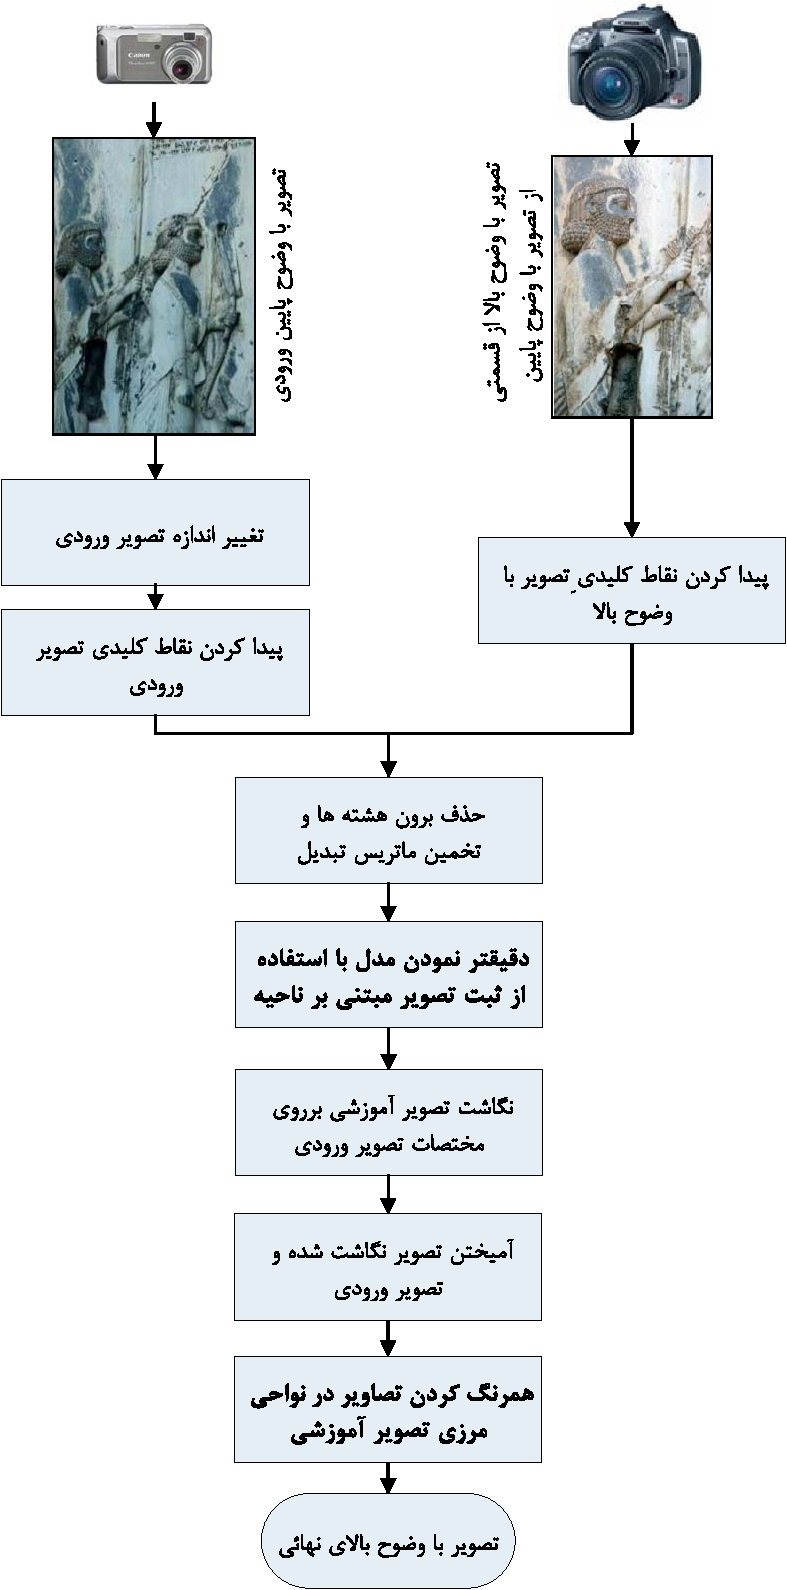
\includegraphics[width=.9\linewidth]{Images/flowchar}
\caption{چارچوب کلی روش پیشنهادی.}
\label{fig:OneLRoneHR}
\end{figure}


\subsubsection{ویژگی‌های بخش تحلیل و ارزیابی}
در صورتی که روش پیشنهادی حسی نبوده ومبتنی بر استدلال ریاضیاتی باشد، می‌توان به ارزیابی عملکرد آن در سامانه و نحوه بهبود نتایج نسبت به کارهای گذشته به طور کمی و کیفی پرداخت. بدیهی است اگر مدل پیشنهادی حسی بوده و قابل استناد ریاضیاتی نباشد، تنها می‌توان به صورت کیفی به ارزیابی عملکرد پرداخت.


\subsection{ویژگی‌های بخش شبیه‌سازی}
\label{Sec:ExperimentalResults}

از آنجایی که بسیاری از تحقیق‌ها به منظور حل‌مساله‌ای عملی پی‌گیری می‌شوند، این بخش از اهمیت خاصی برخوردار است. در این بخش به معرفی شبیه‌سازی صورت گرفته و ارائه نتایج به صورت مطلوب (جدول، نمودار و ...) پرداخته می‌شود. در مواردی که طرح پیشنهادی اثبات شده است، نتایج باید با تقریب خوبی با مدعا یکسان باشد. در مواردی که طرح پیشنهادی اثبات نشده و به طور حسی و مبتنی بر برخی پیش‌فرض‌ها مطرح شده است،  اهمیت این بخش بیشتر از حالت قبل است، چرا که نتایج شبیه‌سازی تنها مستند نویسنده و به نوعی موید مدعای ثابت نشده وی است. این حالت اخیر از دهه آخر قرن بیستم تا کنون به وفور در مقالات معتبر پی‌گیری شده است تا جایی که در صورت تایید نتایج با شبیه‌سازی، آن را به نوعی اثبات برای طرح پیشنهادی در نظر می‌گیرند.

\begin{figure}
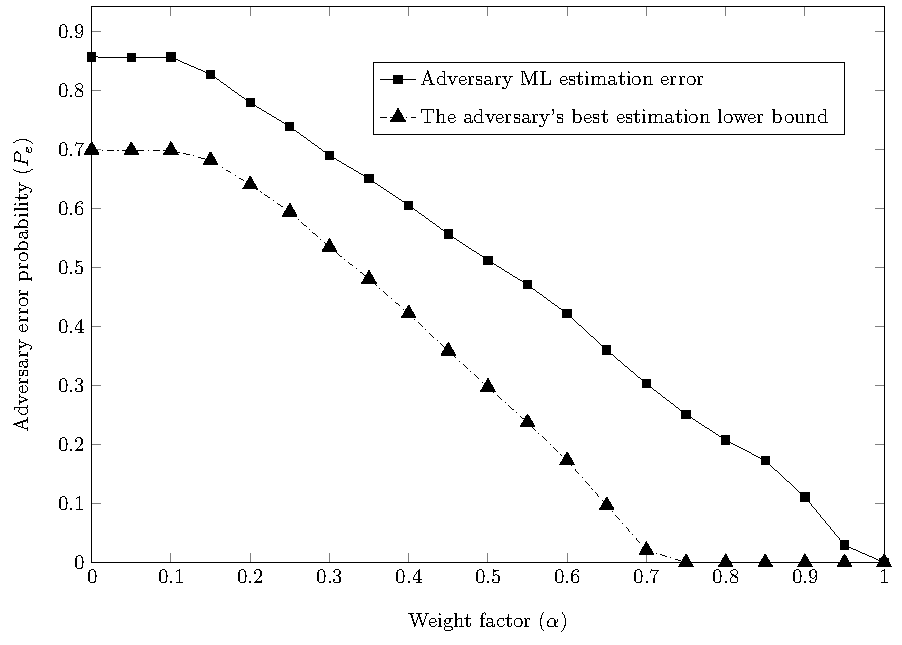
\includegraphics[width=.9\linewidth]{Images/sumXYPlot}
\caption{
زیرنویس نمودارها باید کامل و جامع باشد، به عبارت‌دیگر خواننده بتواند با دیدن نمودار و خواندن زیرنویس آن پی به تمامی اطلاعات نهفته در نمودار ببرد.}
\label{fig:sumXYPlot}
\end{figure}
برای آوردن اشکال در کنار یکدیگر می‌توانید از محیط \lr{subfigure} استفاده کنید. 
\begin{figure*}
\centering
\begin{subfigure}[b]{0.31\textwidth}
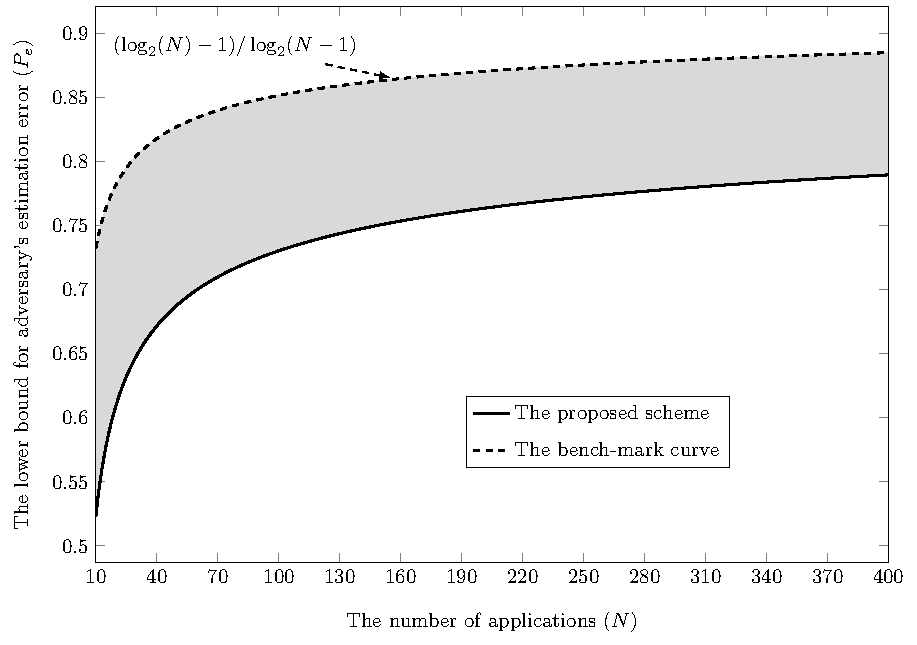
\includegraphics[width=\linewidth]{./Images/famk}
\caption{}
\label{fig:gull}
\end{subfigure}
\begin{subfigure}[b]{0.31\textwidth}
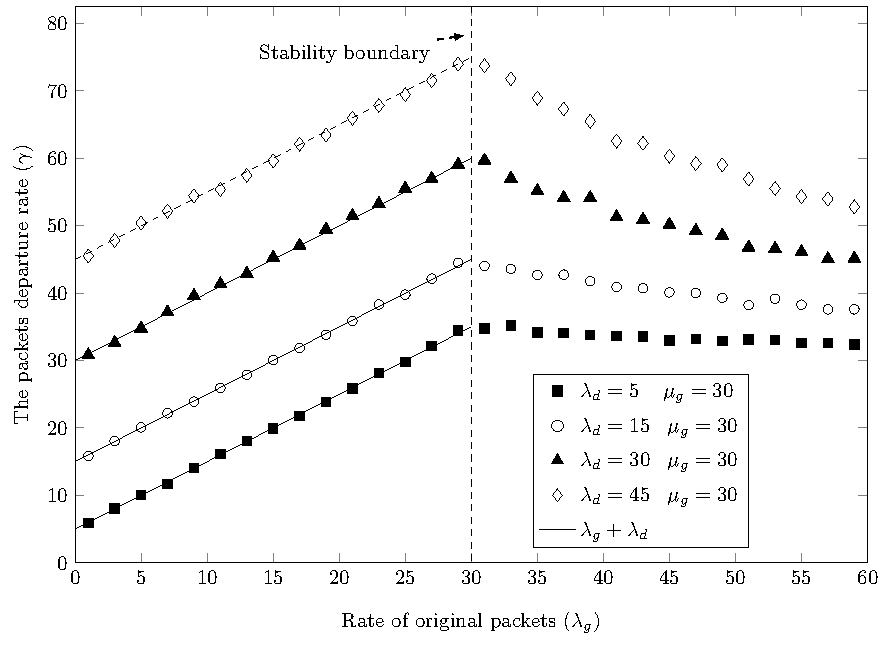
\includegraphics[width=\linewidth]{./Images/saml}
\caption{}
\label{fig:tiger}
\end{subfigure}
\begin{subfigure}[b]{0.31\textwidth}
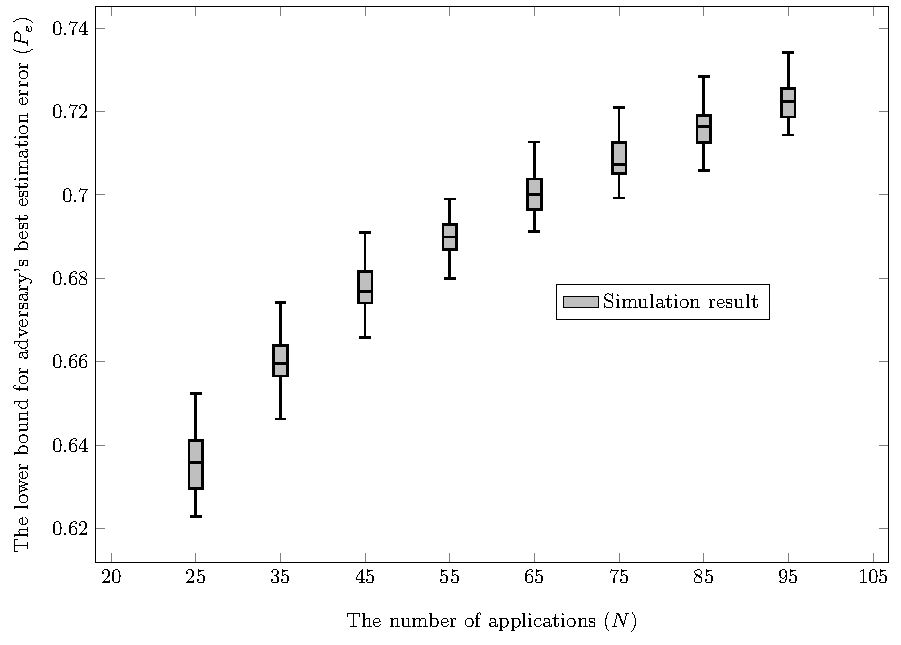
\includegraphics[width=\linewidth]{./Images/EntropyVersus}
\caption{}
\label{fig:EntropyVersus}
\end{subfigure}
\caption{
آ) این شکل در این مورد سخن می‌گوید که .....، ب) در مورد این شکل اکنون صحبت کنید... ، ج) این شکل برای ....
}
\label{fig:animals}
\end{figure*}
در شبیه‌سازی‌ها می‌بایست نویسندگان به صورت دقیق و صریح پیکربندی شبیه‌سازی و مجموعه داده‌ای که مورد استفاده قرار داده‌اند را با ذکر منابع و مراجع مورد نیاز، ذکر کنند. در ضمن پارامترهای مورد استفاده برای شبیه‌سازی باید در همین بخش شبیه‌سازی تعریف شود. به عنوان مثال اگر شما از پارامتر 
\lr{MSE (mean squared error)}
استفاده می‌کنید باید آن را در این بخش تعریف کنید. شکل‌های شبیه‌سازی باید واضح و مشخص باشد. دقت کنید به دلیل این‌که در نهایت مقالات پذیرفته شده به صورت سیاه و سفید چاپ خواهد شد، بدین‌سان از تمایزگذاری با رنگ‌های مختلف بین نمودارها کافی نخواهد بود. یک نمونه از تمایزگذاری مناسب را می‌توانید در نمودار \ref{fig:sumXYPlot} و \ref{fig:tiger} ملاحظه کنید. 

تمامی نمودارهای قسمت شبیه‌سازی باید دارای  \lr{Legend} باشند. محور‌های نمودارها همگی باید دارای برچسب مناسب و همچنین شماره‌گذاری مناسب باشد. در \lr{\LaTeX} سعی کنید نمودارهای خود را با کیفیت \lr{pdf} وارد کنید و از قراردادن نمودارهای  با کیفیت \lr{jpg} و یا کیفیت تصویری خودداری کنید. بسیاری از ابزارهای شبیه‌سازی به شما خروجی \lr{pdf}  را می‌دهند. 

استفاده از نمودارهای نوین به مانند \lr{Box-Plot} به شدت مورد استقبال قرار می‌گیرد. نکته مهم در شبیه‌سازی
انجام پذیرفته در مقاله این است که نویسندگان تنها به گزارش میانگین خطا بسنده کرده‌اند. از دیدگاه علم شبیه‌سازی این کار نمی تواند اطمینان خواننده را به شبیه‌سازی جلب کند. به عنوان مثال دو کلاس را در نظر بگیرید که نمرات سه دانشجوی آن ۹، ۱۰ و ۱۱ است و کلاس دیگر ۵، ۱۰ و ۱۵. هر دو کلاس میانگین یکسانی دارند، اما واقعا بین نمرات این دو کلاس تفاوت زیادی وجود دارد. به عنوان پیشنهاد می توانید از نمودار
\href{https://en.wikipedia.org/wiki/Box_plot}{Box-Plot}
استفاده کنید و یا حداقل بازه اطمینان نتایج را گزارش کنید. نمونه ای از یک \lr{Box-Plot} در شکل
\ref{fig:EntropyVersus}
نشان داده شده است. 

سعی کنید از قرار دادن کدهای شبیه‌سازی چه در قسمت شبیه‌سازی و چه در قسمت روش پیشنهادی به شدت خودداری کنید. نویسندگان به صورت اختیاری می‌توانند کدهای شبیه‌سازی خود را در یک وب‌سایت قرار داده و به آن در مقاله پیوند دهند. 

\subsection{ویژگی‌های بخش نتیجه‌گیری}
در بخش نتيجه، نكات مهم انجام شده در كار بصورت خلاصه مرور و نتايج به دست آمده توضيح داده شوند. همچنين در اين بخش بايد سهم علمي مقاله بصورت واضح بيان شود. هرگز عين مطالب چكيده را در اين بخش تكرار نكنيد. نتيجه می‏‌تواند به کاربردهای پژوهش انجام شده اشاره کند؛ نکات مبهم و قابل پژوهش جديد را مطرح کند؛ ويا گسترش موضوع بحث را به زمينه‏‌های ديگر پيشنهاد دهد.

\subsection{ویژگی بخش پیوست‌ها}
بخش پیوست‌ها یك بخش اختیاری است و شماره‌گذاری  نمی‌شود. موضوع‌های مرتبط با مقاله كه در یكی از گروه‌های زیر قرار گیرند، می‌توانند در بخش ضمایم آورده شوند.
\begin{itemize}
\item
اثبات ریاضی فرمول‌ها یا الگوریتم‌ها.
\item
داده‌ها و اطلاعات مربوط به مطالعه موردی.
\item
نتایج كار دیگر محققان و داده‌های مربوط به مقایسه آن‌ها.
\item
سایر موضوع‌های مرتبط كه جزء بخش‌های اصلی مقاله نباشند.
\end{itemize}


\section{قواعد نگارشی}

شیوایی و رسایی نوشتار در گرو ساده‌نویسی است. تلاش شود در متن مقاله از جملات رسا، گویا، و كوتاه استفاده شود و از نوشتن جملات تودرتو پرهیز شود. به این جمله دقت كنید: «آهنگی كه شما از فروشگاه \lr{iTune} دریافت می‌كنید توسط قالب \lr{DRM} اپل كه یك قالب فایل \lr{AAC} انحصاری و محافظت شده است كه اپل مجوز استفاده از آن را به هیچ كس نمی‌دهد، محافظت می‌شود». این جمله در واقع از سبك نگارش زبان انگلیسی پیروی می‌كند و به هیچ وجه برای جملات پارسی مناسب نیست. به راحتی می‌توان این جمله را به این صورت بازنویسی كرد: «آهنگی كه شما از فروشگاه \lr{iTune} دریافت می‌كنید توسط قالب \lr{DRM} اپل محافظت می‌شود. این قالب یك قالب فایل \lr{AAC} انحصاری و محافظت شده است، و اپل مجوز استفاده از آن را به هیچ كس نمی‌دهد».

جداسازی اجزای مختلف یك جمله نیز نقش زیادی در فهم آسان آن دارد. ویرگول می­تواند اجزای یک جمله را در جایی که نیاز به مکث هست، ازهم جدا کند؛ حال آن که نقطه ویرگول برای جداسازی دوجمله که با هم ارتباط معنایی دارند، بکار می­رود. نقطه نیز برای جدا كردن جملات مورد استفاده قرار می­گیرد. درکاربرد هلالین (پرانتز) باید توجه شود که عبارت داخل آن برای توضیحی است که از اجزای جمله محسوب نشده و درصورت حذف خللی به آن وارد نمی­شود. درمقابل، گیومه برای برجسته کردن جزیی از جمله بکار می­رود.

تا جای ممكن از بكار بردن كلماتی مثل «می­باشد»، «گردید»، و «بوده باشد» پرهیز شود. به جای آن‌ها اغلب می‌توان از كلمات ساده و روان مثل «است» و «شد» استفاده كرد. بكارگیری كلمات دشوار و غیرمعمول تنها باعث پیچیده شدن جمله و دشوار شدن فهم آن می‌شود.

برای كلمات فنی تا حد امكان از معادل‌های پارسی استفاده شود. بدون تردید كلمه «پردازش» زیباتر از «پروسس» است، و یا كلمه «ریزپردازنده» از «میكروپروسسور» مناسب‌تر است. در چنین مواقعی اگر احتمال می‌دهید خواننده با معادل پارسی آشنا نیست، از پانویس برای نوشتن معادل انگلیسی استفاده كنید. این كار را در اولین كاربرد معادل‌های پارسی انجام دهید. مثل گره راهنما\LTRfootnote{Anchor Node}

تا حد امكان از كلمات انگلیسی در جملات استفاده نكنید. مثلاٌ بجای نوشتن \lr{Microsoft} می­توانید بنویسید: «میكروسافت». اگر ناچار شدید در یك جمله از كلمات انگلیسی استفاده كنید، حتماً فاصله كافی بین آن‌ها و كلمات پارسی را رعایت كنید.

\subsection{علامت‌گذاری}
برای خوانایی بهتر مقاله باید سعی شود تا حد امكان علامت­گذاری متن مقاله بدرستی انجام شود. دقت كنید تمام علامت‌هایی مثل نقطه، ویرگول، نقطه ویرگول، دونقطه، و علامت سوال باید به كلمه قبل از خود چسبیده باشند، و از كلمه بعدی تنها به اندازه یك فضای خالی فاصله داشته باشند. علامت خط تیره باید به اندازه یك فضای خالی از كلمه قبل و بعد از خود فاصله داشته باشد؛ مگر این كه كلمه قبلی یا بعدی یك عدد باشد، كه در این صورت باید به آن بچسبد. بین كلماتی كه جدا هستند باید یك فضای خالی فاصله باشد.
\subsection{املا}
درستی نوشتار بر پایه املای زبان پارسی ضروری است. در این بخش برخی از موارد اشتباه متداول را یادآوری می‌كنیم. می‌توانید اطلاعات دقیق‌تر را با مراجعه به كتاب­های نوشته شده در این زمینه پیدا كنید.

در افعال حال و گذشته استمراری باید دقت شود كه «می» از جزء بعدی فعل جدا نماند. برای این منظور می‌توانید از نیم‌فاصله استفاده کنید.

در مورد «ها»ی جمع نیز دقت كنید كه از كلمه جمع بسته شده جدا نوشته شود؛ مگر در كلمات تك هجایی مثل «آنها». برای جدانویسی نیز از فاصله متصل استفاده كنید. مثلاٌ «پردازنده ها» را بصورت «پردازنده‌­ها» بنویسید.

جمع بستن كلمات پارسی یا لاتین با قواعد زبان عربی اشتباه است. بنابراین «پیشنهادات» و «اساتید» اشتباه و درست آنها «پیشنهادها» و «استادان» است.

بهتر است همواره حرف اضافه «به» از کلمه بعدی خود جدا نوشته شود، مگر آن که این حرف جزء یک فعل یا صفت یا قید باشد؛ مانند: «بکار بستن»، «بجا» و «بندرت».

در مورد کلمات حاوی همزه قواعدی وجود دارد که پرداختن به آنها دراین مقاله نمی­گنجد، اما برای نمونه به املای کلمات «مسأله»، «منشأ» و «رئیس» دقت كنید. همچنین، همزه در انتهای کلماتی که به الف ختم می­شوند، نوشته نمی­شود و درصورت اضافه شدن به کلمه بعدی، از «ی» استفاده می­شود: «اجرا شده»، و «اجرای برنامه».


\subsection{شكل‌ها و جدول­ها}
شكل‌ها و جدول­ها باید دارای عنوان باشند. عنوان شكل‌ها در زیر شكل و عنوان جدول­ها در بالای جدول قرار می‌گیرند. در صورتی كه از شكل‌ها یا جدول­های سایر منابع استفاده می‌كنید، باید حتماً شماره آن مرجع را در عنوان شكل یا جدول ذكر كنید.

در هنگام ارجاع به شكل یا جدول از شماره آن استفاده كنید و از بكار بردن عباراتی همچون «شكل زیر» پرهیز كنید. تمام جدول­ها و شكل‌ها باید در متن مورد ارجاع قرار گیرند. 


\subsection{ فرمول‌ها و عبارات ریاضی}
برای هر فرمول باید یك شماره در نظر گرفته شود. این شماره را در داخل یك جفت هلالین و بصورت راست‌چین قرار دهید.  در   \lr{\LaTeX}  شماره گذاری به صورت خودکار انجام می‌پذیرد. تمام متغیرها، پارامترها، و نمادهای یك عبارت ریاضی باید توضیح داده شوند. اگر قبل از نوشتن فرمول این كار انجام نشده است، باید بلافاصله پس از فرمول این توضیحات بیان شوند. مثال زیر را در نظر بگیرید.

اگر $\rho$ بیانگر چگالی تخمینی باشد، خواهیم داشت:
\begin{equation}
\rho = \frac{m}{A},
\end{equation}
كه درآن  $m$ جرم تخمینی و $A$ سطح آن است. 

اگر در مقاله شما نمادهای ریاضی متنوعی مورد استفاده قرار می‌گیرد، حتما سعی کنید جدول نمادها در متن خود داشته باشید. مثل جدول \ref{tab:symbols}.
\begin{table}[H]
\centering
\caption{نمادهای مورد استفاده در  مقاله}
\label{tab:symbols}
\begin{tabular}{cp{6cm}}\hline
نماد & توضیحات
\\\hline
$N$ &
تعداد کل گره‌های شبکه
\\
$\mathbb{R}^{++}$ &
مجموعه اعداد حقیقی مثبت بزرگتر از صفر
\\
$\rho_{t}$ &
چگالی شبکه در لحظه $t$
\\
$\mathrm{Pr}[A]$ &
احتمال رخداد رویداد $A$
\\
\hline
\end{tabular}
\end{table}







\section{نکاتی در مورد نوشتن مقاله با \lr{\LaTeX}}


نویسندگانی که با محیط \lr{\LaTeX} و نحوه کار با آن آشنایی ندارند می‌توانند به سایت
\url{www.parsilatex.com}
مراجعه کنند. مطالب مفید بسیاری در این زمینه در سایت مذکور قرار داده شده است. همچنین تمامی سوالات و اشکالات مرتبط با این استایل  و در حالت کلی مرتبط با \lr{\LaTeX} را می‌توانید در تالار پرسش و پاسخ همین سایت مطرح نمایید.  

برای کار با این استایل در ابتدا چندین گام را می‌بایست بردارید:
\begin{enumerate} 
\item
نصب یک کامپایلر به مانند \lr{TeXLive}. دقت کنید این استایل را می‌توانید توسط
\lr{TeXLive 2014} ویا \lr{TeXLive 2015}
بروز شده استفاده نمایید. برای  دانلود \lr{TeXLive} می‌توانید به
\href{www.tug.org/texlive/}{سایت \lr{TeXLive}}
مراجعه کنید. در ضمن قابلیت خرید اینترنتی و ارسال پستی این مجموعه از طریق سایت \lr{parsilatex.com} نیز فراهم شده است، بدین منظور به آدرس زیر مراجعه کنید.

\href{http://parsilatex.com/site/product/%D9%85%D8%AC%D9%85%D9%88%D8%B9%D9%87-%D9%BE%D8%A7%D8%B1%D8%B3%DB%8C%E2%80%8C%D9%84%D8%A7%D8%AA%DA%A9/}{
بخش خرید سایت پارسی‌لاتک}


\item
نصب یک ویرایشگر مناسب برای زبان فارسی به مانند \lr{TeXStudio}.
\item
نصب فونت‌های \lr{IRMitra} و \lr{Times New Romans}.
\item
کامپایل فایل نمونه ارایه شده. نویسندگان در صورتی سه گام قبلی را با موفقیت پشت‌سر گذاشتند که بتوانند فایل نمونه قرار داده شده را با موفقیت و به صورت \lr{Normally} کامپایل کنند. 
\end{enumerate}
لازم به ذکر است که تمامی عبارت‌ها و کلمات انگلیسی در فایل \lr{\LaTeX} باید درون دستور \lr{lr} قرار گیرند. مثلا:
\lr{Support vector} و یا \lr{Machine Learning}.
دقت کنید که تمامی کلمات و عبارت‌های اختصاری می‌بایست در اولین فراخوانی به صورت باز شده ارایه شود. به عنوان مثال در اولین مکانی که شما از کلمه اختصاری  \lr{SVM} استفاده می‌کنید باید آن را به صورت 
\lr{SVM (support vector machine)}
بنویسید. به صورت معمول تمامی حروف حالت بازشده باید با حرف کوچک نوشته شود.

ترجیحا توصیه می‌شود که نویسندگان از قراردادن پاورقی در مقاله پرهیز کنند، اما در صورت نیاز شما می‌توانید با دستور \lr{footnote} پاورقی فارسی و با دستور \lr{LTRfootnote} پاورقی انگلیسی قرار دهید. مثل: در این روش\footnote{در واقع منظور ما ...} و یا حسگر\LTRfootnote{Sensor}. دقت کنید که همه پاورقی‌ها در انتهای متن در بخشی به نام پانویس چاپ خواهند شد و نه در همان صفحه.

در صورتی که می‌خواهید بر روی یک کلمه و یا عبارت در یک متن تاکید کنید، لطفا از دستور \lr{emph} استفاده کنید، مثل: کار اصلی ما در این مقاله ارایه یک روش
\emph{داده‌کاوی}
است. تقریبا تمامی بسته‌های مورد نیاز برای نوشتن یک مقاله در استایل \lr{\LaTeX} تهیه شده قرار داده شده است. اما در صورت نیاز به یک بسته معین لطفا استایل قرار داده شده را تغییر دهید و قبل از فراخوانی بسته‌های \lr{hyperref} و بسته \lr{\XePersian} بسته خود را وارد کنید. در هنگام آپلود مقاله نیز کل فایل‌های \lr{\LaTeX} باید به صورت \lr{zip} شده در سایت مورد نظر قرار داده شود. محتویات فایل با پسوند \lr{zip} باید شامل خروجی \lr{pdf}، تمامی تصاویر، فایل اصلی \lr{tex}، فایل با پسوند \lr{bib} و هر فایل دیگر مورد نیاز باشد.

برای نوشتن فرمول یک خطی در \lr{\LaTeX} به سادگی می‌توانید از محیط \lr{equation} استفاده کنید. مثل:
\begin{equation}
A = B^2 + \frac{\gamma}{4}.
\label{eq:dols}
\end{equation}
روابط می‌بایست در صورت نیاز حتما شماره‌گذاری شوند. برای عدم شماره‌گذاری می‌توانید از محیط \lr{equation*} بهره بگیرید.مثل:
\begin{equation*}
A = \frac{\gamma}{\zeta}, \quad\quad \gamma\in\mathbb{R}^{++}.
\end{equation*}
برای روابط چندخطی از محیط \lr{align} استفاده کنید. مثل:
\begin{align}
A =& B^c+\alpha \nonumber\\
R =& A + T.
\label{eq:sams}
\end{align}
و یا به عنوان مثال دیگر:
\begin{align}
\mathrm{H}(\lambda_{g}|\lambda_{g}+\lambda_{d})  =& \frac{1}{N}\sum_{i=1}^{N}\log_{2}(N-i+1) \nonumber\\
&+  \frac{1}{N}\sum_{i=1}^{N}\frac{\sum_{j=i}^{N}\log_{2}(\Upsilon_{N}-\Upsilon_{N-j})}{N-i+1}, \nonumber\\
=& \sum_{i=1}^{N}\frac{\sum_{j=i}^{N}\log_{2}(\Upsilon_{N}-\Upsilon_{N-j})}{N(N-i+1)}.
\label{eq:conditionalentorpyresult}
\end{align}


برای ارجاع به روابط و فرمول‌ها نیاز نیست بنویسید مثلا فرمول شماره ..، فقط کافی است که برچسب فرمول را با دستور \lr{eqref} فراخوانی کنید. در این صورت نیازی به قرار دادن پرانتز نیست و \lr{\LaTeX} به صورت خودکار پرانتزها را می‌گذارد. مثلا با قرار دادن \eqref{eq:sams} در \eqref{eq:dols} خواهیم داشت ... 

سعی کنید مطالب خود را به صورت منظم در قالب تعدادی تعریف، قضیه، لم و گزاره بیاورید. تمامی این محیط‌های در استایل آماده شده تعریف شده است و براحتی قابل استفاده است.
\begin{definition}[حالت پایدار]
حالتی را پایدار گوییم که در آن تغییر آمارگان پارامترهای صف برابر صفر باشد. اگر $‎\varpi$ را یک پارامتر صف در نظر بگیریم، خواهیم داشت.
\begin{equation}
\frac{\mathrm{d}\varpi(t)}{\mathrm{d}t}=0
\end{equation}
\end{definition}
\begin{theorem}[پایستگی جریان]
در صورتی که سامانه مورد بررسی ‎ارگودیک‎ و در ‎پایدار‎ باشد، آن‌گاه نرخ ورود بسته به سامانه همواره برابر با نرخ خروج آن خواهد بود. 
\label{theorem:jddkssskaa}
\end{theorem}
\begin{theorem}
قرار دادن نام برای قضیه به مانند قضیه قبل که نامش پایستگی جریان بود اختیاری است.
\label{theorem:jdtysssaa}
\end{theorem}
\begin{proof}
سعی کنید اگر قضیه برای مرجع دیگری است اثبات آن را در مقاله نیاورید و فقط به مرجع مذکور ارجاع دهید. اگر اثبات در روند مقاله اهمیت دارد آن را درون متن مقاله بیاورید. اما اگر در روند کلی تاثیری ندارد اثبات را به قسمت پیوست‌ها ببرید. 
\end{proof}
\begin{corollary}
در یک صف نرخ ورود با خروج برابر است.
\end{corollary}
\begin{corollary}
در یک سامانه نرخ ورود برابر است با تعداد بسته‌ها ....
\end{corollary}
\begin{lemma}
   اگر $N_t$ نشان‌دهنده تعداد بسته رسیده تا زمان $t$ به .......
\begin{equation}
P(t_{i}>t)=P(N(t)<i)\Longrightarrow P(t_{i}<t)=1-
\end{equation}

\end{lemma}%%
\begin{lemmaproof}
برای اثبات به مرجع .... برای اثبات قضایا از محیط \lr{proof} و برای اثبات لم‌ها از محیط \lr{lemmaproof} استفاده کنید.
\end{lemmaproof}

\begin{principle}[عدم قطعیت]
برطبق اصل عدم قطعیت هر ذره ....
\end{principle}

توصیه می‌شود که نویسندگان برای نمادهای ریاضیاتی سعی کنند از نمادهای ساده و استاندارد استفاده کنند. به عنوان مثال مجموعه اعداد حقیقی را بهتر است به جای $R$ با $\mathbb{R}$ نشان داد. تمامی عملگرهای ریاضیاتی به مانند عملگر امیدریاضی، آنتروپی، احتمال رخداد یک رویداد باید به صورت غیرایتالیک نوشته شود، مثل:
$\mathrm{E}[..]$, $\mathrm{Pr}[..]$, $\mathrm{H}[..]$ و ... . 

نویسندگان می‌بایست حتما و حتما نمادها و روابط ریاضی موجود در متن را در حالت \lr{math mode} بنویسند و نه در حالت متنی. به عنوان مثال به جای \lr{A+B} که به صورت متنی است، بهتر است بنویسید $A+B$.
\section{نتیجه گیری}
در این بخش نویسندگان باید به صورت خلاصه کل روندی که در مقاله پیموده شده است را توضیح دهند. در ضمن نویسندگان می‌توانند در این بخش ایده‌های جدید برای توسعه هرچه بیشتر و بهتر مقاله خود را مطرح کنند.

\section*{سپاس‌گزاری}
بخش سپاسگزاری در صورت نیاز بصورت كوتاه و در یك بند آماده شود. بخش سپاسگزاری دارای شماره نیست. در این قسمت نویسندگان می‌توانند از افراد و یا نهادهای پشتیبان و یاریگر تشکر و قدردانی کنند. از همین مجال استفاده می‌شود و از همه دوستانی که در روند برگزاری کنفرانس و تهیه این استایل یاریگر ما بودند، تشکر و قدردانی به عمل می‌آید، به خصوص آقایان وفا خیلقی نویسنده بسته ارزشمند \lr{\XePersian}، محمد امین طوسی، امیر حسین رضایی تبار، وحید دامن‌افشان، فرشاد ترابی و دیگر دوستان در سایت پارسی‌لاتک.

\section*{پیوست‌ها}
بخش پیوست‌ها یك بخش اختیاری است و شماره‌گذاری  نمی‌شود. موضوع‌های مرتبط با مقاله كه در یكی از گروه‌های زیر قرار گیرند، می‌توانند در بخش ضمایم آورده شوند.
\begin{itemize}
\item
اثبات ریاضی فرمول‌ها یا الگوریتم‌ها.
\item
داده‌ها و اطلاعات مربوط به مطالعه موردی.
\item
نتایج كار دیگر محققان و داده‌های مربوط به مقایسه آن‌ها.
\item
سایر موضوع‌های مرتبط كه جزء بخش‌های اصلی مقاله نباشند.
\end{itemize}


\bibliography{lib}

\theendnotes
\end{document}


